\chapter{Literature review}
\label{ch:Literature}

Taking into account the objectives of this work, this chapter presents the theoretical foundation. First, topics related to the educational environment are presented to understand the context in which this work is inserted. Secondly, ways to visualize educational data are cited to show successful examples of applications in this field. Finally, the basic concepts in data analysis are displayed as they are important to understand the experiments and results produced in this research.

\section{Semi-presential courses}

Semi-presential courses, hybrid education, or flexible education are terms that refer to educational models that combine activities from distance, usually on the Internet, with face-to-face interaction \cite{camilloo2010interaccao}.

\cite{bacich2015ensino} defines hybrid learning as a pedagogical approach that combines classroom activities and actions made with the help of digital technologies. Its main strategy is to put the focus of the learning process on the student and not on the traditional way in the classroom. With this method, the material and instructions about a class are not transmitted by the teacher but are used by the student in different environments. This way the classroom becomes a place to actively learn, by problem solving, discussions, use of labs, and collaboration with teacher and other students.

The idea behind mixing online and offline learning are that learning is not just a one-time event but a continuous process. Blending learning provides numerous benefits overusing any single learning medium alone. Programs that use this education method can include various forms of learning tools, such as real-time virtual software, self-paced web courses, and knowledge management systems \cite{singh2021building}.

Hybrid education can already be considered a big bet to the learning process in the 21st century. Given this model that unifies the best practices of virtual and presential learning, the universities can revolutionize the ways of teaching and learning \cite{de2021ensino}.

This type of learning has some advantages, such as (1) individual student monitoring, (2) better time organization of class activities, (3) time and space flexibility for the student, (4) feedback from the teacher and other classmates, (5) quality material for the course, and (6) collaboration and communication in the virtual learning environment. But it can also offer some challenges, such as (1) coordination between the online and the presential components of the course, and (2) possible difficulty in adaptation to this model of learning \cite{nunes2016learning}.

The Moodle\footnote[1]{\hspace{1mm}\url{https://moodle.org/}} system is an example of an open-source tool commonly used in mixed learning. Moodle is a virtual learning environment that has functionalities such as (1) allows teachers to release files in different formats, practice tests, and exams and set the time and way that the students have permission to use that material and make those practice tests and exams; (2) tools that help with communication such as forums and chats; (3) profile management, allowing a system with limited access to each user based on its profile; (4) score management to allow the teacher to grade every activity. All these services and the fact that Moodle is available in various languages make it a system frequently used \cite{lopes2007ambientes}.

\section{Educational early warning systems}

Early warning systems can be thought of as the next step in the prediction of academic performance. This type of system aims to predict academic performance at an early stage using features given by online learning settings. Teachers may then be able to identify students at risk of academic failure and offer to help these students make improvements \cite{akccapinar2019using}.

The Signal Project, developed at Purdue University, is often cited as a case of a successful early warning system. This system makes use of the data collected by instructional tools to enable faculty to provide feedback to students based on predictive models. Based on the result of the systems' algorithm, a red, yellow, or green signal is displayed at the student’s course homepage. Red indicates a high likelihood of being unsuccessful, yellow indicates a potential problem of succeeding, and green demonstrates a high likelihood of succeeding in the course (see figures \ref{fig:s1} and \ref{fig:s2}). \cite{arnold2012course}.

\begin{figure}[htb]
	\centering
  	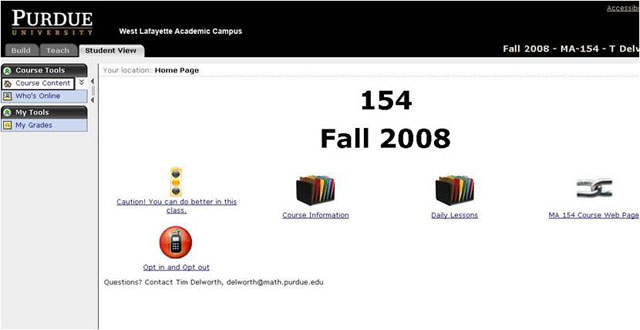
\includegraphics[scale=1]{Imagens/signals1.jpg}
  	\caption{Student dashboard (source: \cite{arnold2010signals})}
  	\label{fig:s1}
\end{figure}

\begin{figure}[htb]
	\centering
  	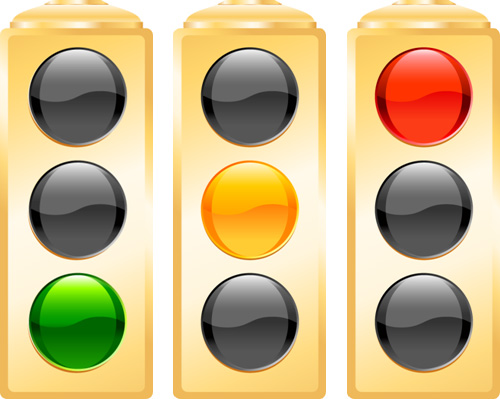
\includegraphics[scale=.3]{Imagens/signals2.jpg}
  	\caption{Traffic signals (source: \cite{arnold2010signals})}
  	\label{fig:s2}
\end{figure}

Another example of usage of these alert systems is in \cite{shi2014developing}, the authors suggest an early warning system be used as a plugin to a learning management system\abrv{Learning Management System}{LMS}(LMS). After a student logs into the LMS (see figure \ref{fig:lms}), a dashboard with his/her current learning status is displayed (on the left side of the screen).

In addition, there is also a list of the key performance indicators, these indicators are the most important features that were calculated by the data mining engine. For each indicator, the student can see the learning history (on the right side of the screen). This learning history can also be compared with the results of the class. All of these elements can help students to monitor their performance. Thus, the system can help with the identification of at-risk students at any point in time, greatly minimizing the negative effects of poor performance.

\begin{figure}[htb]
	\centering
  	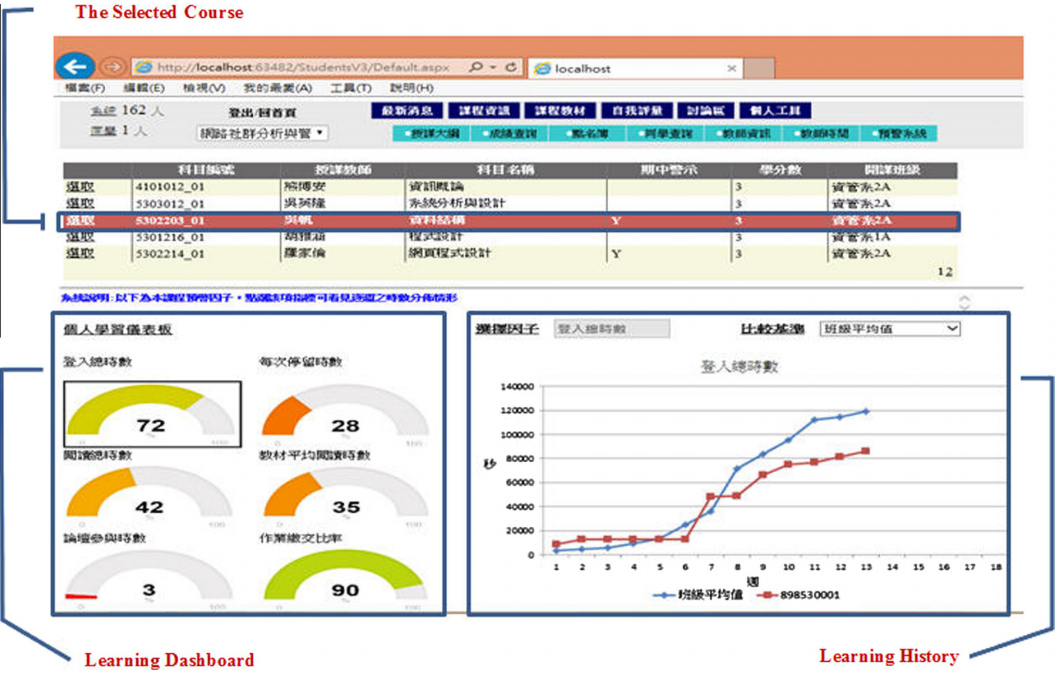
\includegraphics[scale=.5]{Imagens/lms.png}
  	\caption{Student dashboard (source: \cite{shi2014developing})}
  	\label{fig:lms}
\end{figure}

Studies show that early prediction of academic performance can be done, but the development of a generic prediction model, to be used in different courses, is a challenging task. One big reason behind this is that the different instructional conditions used in the course affect the performance of prediction models. Thus, it is important to develop and validate prediction models for each different course \cite{akccapinar2019using}.

\section{Educational data mining (EDM)}
\label{sc:edm}

EDM is a research field that applies statistics and machine learning algorithms over data generated in an educational context, to solve educational related issues. Hence, it is interested in developing methods to explore the data in an educational setting and, using these methods, to better explain students and the environment in which they learn \cite{romero2010educational}.

The four main steps of the EDM process are the following \cite{sokkhey2020developing}, \cite{romero2020educational}:

\begin{enumerate}
    \item Obtain raw data
    
    In this first step, the targeted data is collected from sources as school databases or questionnaires. The are multiple types of data that can be used: educational (e.g., navigation in the virtual environment, quizzes, exercises, forum messages, etc.) administrative data (e.g., information about the school, teachers, curriculum, disciplines), demographic data (e.g., city, gender, school type, income, age, etc.), student emotions (e.g., motivation, emotional states), and so on.
    
    There are also different granularity levels (from crude to refined) or various levels of hierarchy (answer level, session-level, student level, classroom level, and school level) that can provide more or fewer data.
    
    \item Preprocessing
    
    Since the raw data can come from several different sources and have distinct formats, it is often the case that the data needs to be processed to achieve the desired format. This step also includes choosing what data to collect, making sure the data is aligned with the questions the work intends to answer. Some examples of techniques are: 
    \begin{itemize}
        \item Dealing with missing data: to handle the problem of having instances with missing values in the data set, an option is to fully discard those instances, or replace the missing values with the most frequent/average value.
        \item Discretization: transforms some continuous variable onto discrete values.
        \item Feature engineering: selecting the most important variables or creating new attributes from already existing ones.
        \item Feature scaling: some algorithms need the data to be shaped in a specific way. A few examples are:
        \begin{itemize}
            \item Normalization: scales the features in a predetermined range (usually the 0-1 interval).
            \item Standardization: scales the data to follow a normal distribution (usually with 0 mean and 1 standard deviation).
        \end{itemize}
    \end{itemize}
    
    \item EDM methods
    
    There is a wide range of traditional Data Mining\abrv{Data Mining}{DM}(DM) methods that can be used in this step for solving educational problems, such as visualization, prediction, clustering and social network analysis. Table \ref{tab:edm-methods} gives more examples and details about these methods.
    
    \item Interpretation
    
    The last step brings new knowledge discovered by the EDM methods to be used by teachers and students to make interventions to improve student learning performance. That is, taking action is the final goal of any learning analytics process and the outcome of follow-up actions will determine the success or failure of the analytical attempts. It is also important that the models generated in the previous step are comprehensible to be useful for those who will use the model. In this context, visualization techniques can be very useful for showing results in a way that is easier to interpret.
\end{enumerate}


\begin{table}[htb!]
\centering
\begin{tabular}{lll} \hline
\textbf{Method} & \textbf{Goal/description} & \textbf{Applications} \\ \hline
Causal mining & \begin{tabular}[c]{@{}l@{}}To find causal relationship or\\ patterns in data.\end{tabular} & \begin{tabular}[c]{@{}l@{}}Finding what attributes of\\ students' behavior cause\\ learning, academic failure,\\ and so on.\end{tabular} \\ \hline
Visualization & To show a graphical view of data. & \begin{tabular}[c]{@{}l@{}}Data visualizations tools\\ that help inform results of\\ EDM research\\ to educators.\end{tabular} \\ \hline
Prediction & \begin{tabular}[c]{@{}l@{}}To infer a target variable\\ from some combination\\ of other variables.\\ Classification and regression\\ are examples of\\ prediction methods.\end{tabular} & \begin{tabular}[c]{@{}l@{}}Predicting student\\ performances.\end{tabular} \\ \hline
Clustering & To group similar students. & \begin{tabular}[c]{@{}l@{}}Grouping similar\\ materials or students\\ based on their \\ learning patterns.\end{tabular} \\ \hline
\begin{tabular}[c]{@{}l@{}}Social network\\ analysis\end{tabular} & \begin{tabular}[c]{@{}l@{}}To analyze the social relationships\\ between individuals in a network.\end{tabular} & \begin{tabular}[c]{@{}l@{}}Analysis of the structure\\ and relations\\ in collaborative tasks.\end{tabular} \\ \hline
Recommendation & \begin{tabular}[c]{@{}l@{}}To calculate the rating\\ or preference\\ a user would give to an item.\end{tabular} & \begin{tabular}[c]{@{}l@{}}To make recommendations\\ to students related to their\\ activities, tasks, links to visit,\\ problems to solve\\ or courses to take, and so on.\end{tabular} \\ \hline
Outlier detection & \begin{tabular}[c]{@{}l@{}}To identify significantly\\ different individuals.\end{tabular} & \begin{tabular}[c]{@{}l@{}}Detection of students with\\ learning difficulties.\end{tabular} \\ \hline
Statistics & \begin{tabular}[c]{@{}l@{}}To calculate descriptive and\\ inferential statistics.\end{tabular} & Interpreting educational data. \\ \hline
Text mining & \begin{tabular}[c]{@{}l@{}}To extract information\\ from text.\end{tabular} & \begin{tabular}[c]{@{}l@{}}Analyzing the contents\\ of documents, chats,\\ forums and web pages.\end{tabular} \\ \hline
\end{tabular}
\caption{Popular EDM methods (adapted from \cite{romero2020educational})}
\label{tab:edm-methods}
\end{table}

An overview of the EDM knowledge discovery cycle can be seen in figure \ref{fig:edm}. It shows how this method works as a cycle that aims to continuously improve the educational environment, by using the educational data to create models to be used by learners and academic authorities in an educational setting.

\begin{figure}[htb]
	\centering
  	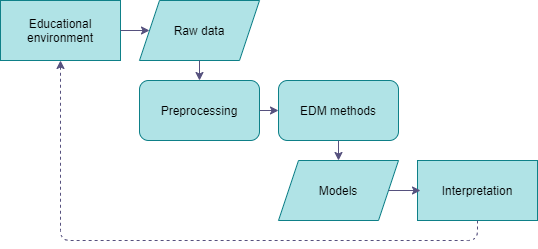
\includegraphics[scale=.7]{Imagens/edm.png}
  	\caption{EDM knowledge discovery cycle (adapted from \cite{linan2015educational})}
  	\label{fig:edm}
\end{figure}

\section{Predictive analysis}

Predictive analysis is an example of a DM method that aims to estimate the value of some feature of the data set. When this value is numerical or continuous we have a regression task, when it is categorical or discrete, a classification task. Details about this method are presented in the following section \ref{sc:class}.

\subsection{Classifiers}
\label{sc:class}

Classification is one of the possible approaches to DM, where the goal is to create classification models using the training data so that results can be predicted into one of the classes of the data. The following subsections were made following the works of \cite{bramer2007principles} and \cite{larose2006data}, and it displays some examples of classifiers presented in more detail.

\subsubsection{$k$-Nearest Neighbors (KNN)}

The\abrv{$k$-Nearest Neighbors}{KNN}KNN algorithm classifies new instances based on the \emph{closeness} to the instances that already are in the data set. For example: in a 3-NN classifier each newly added instance is classified by the votes of the 3 nearest neighbors. This voting system can be a simple best of 3 or it can weigh the votes by distance, meaning that closer neighbors will receive greater weight than the classifications of more distant ones. This classifier is used mainly when all attribute values are continuous, although it can be altered to handle categorical attributes. 
KNN is an example of a lazy learning algorithm because it uses all the data for training. Thus, it does not have a specialized training phase.

About the distance measures, there are two common ways of doing it:

\begin{itemize}
    \item Euclidean Distance: it is the default way of measuring point distance in a plane. Formally, the distance $d$ between points $a$ and $b$ in $n$ dimensions is:

    \begin{equation}d(a,b) = \sqrt{\sum_{i=1}^n {(a_i - b_i)}^2}\end{equation}

    \item Manhattan Distance: it measures the distance between two data points in a grid like way. Formally, the distance $d$ between points $a$ and $b$ in $n$ dimensions is:
    
    \begin{equation} d(a,b) = \sum_{i=1}^n {|a_i - b_i|} \end{equation}
\end{itemize}

Alternatively, any other method that respects the requirements of distance measures can be used. Using the notation $d(a,b)$ to stand for the distance between points $a$ and $b$, these conditions are:

\begin{enumerate}
    \item $d(a,a) = 0$, meaning that the distance of any point $a$ to itself is zero.
    \item $d(a,b) = d(b,a)$ is the symmetry condition. In other words, the distance from $a$ to $b$ is the same as from $b$ to $a$.
    \item $d(a,b) \le d(a,c) + d(c,b)$ is the triangle inequality. It captures the idea that 'the shortest distance between any two points is a straight line'.
\end{enumerate}

It is important to notice that these ways of measuring distance can work badly if the data is not in the same range of values. This happens because large values will weigh more than small ones. So, before running the classifier it is critical to normalize the features.

In real problems, a common value for K is the square root of the data set size. Also, an odd value for K is desired to avoid confusion between the two classes. If it is chosen K values that are low, the results should be less biased but with higher variance, but when the K values are high, the results should have less variance and higher bias. This is what is called the \emph{bias–variance dilemma}. In other words, it is the conflict in trying to minimize those two types of error simultaneously.

In summary, the algorithm for the KNN classifier is:

\begin{algorithm}[H]
Step 1 - find the k \emph{closest} instances to the new instance. \\
Step 2 - use a voting system to choose a class from these k instances as the result.
\caption{KNN}
\end{algorithm}

\subsubsection{Naive Bayes}

Naive Bayes is a set of classifiers that uses concepts of probability theory to find the most likely possible classification for each new instance. The algorithm combines prior probability and conditional probabilities into a formula that can calculate the probability of each class. Prior probability is defined as the probability of an event before new data is collected, and conditional probability is the probability of an event occurring, given that another event happened. These concepts are the basis for the Bayes' theorem, formally defined as:

\begin{equation} P(A|B) = \frac{P(B|A)P(A)}{P(B)} \end{equation}

Where A and B are events, and P(X) is the probability of some X event. P(A) is called \emph{priori} or prior probability of A, and P(A|B) is a \emph{posteriori} probability of B, meaning the probability of a event after some evidence is seen.

Formally, a Bayes classifiers' definition is: given a set of $n$ classes $c_1$, $c_2$, ..., $c_n$, which have prior probabilities $P(c_1)$, $P(c_2)$, ..., $P(c_n)$, respectively, and m features $a_1$, $a_2$, ..., $a_m$, and given a new instance with features' values $v_1$, $v_2$, ..., $v_m$, the probability of each class will be proportional to:

\begin{equation} P(c_i) \times \prod_{j=1}^m P(a_m=v_m | class = c_i) \end{equation}

Finally, the class for each new instance will be stated as the class with higher probability.

The formula above assumes that all attributes are independent (hence the \emph{naive} in the methods' name). Another restriction is that this formula works only with categorical features. To overcome this, a specific type of Bayes classifier must be used: Gaussian Naive Bayes, where continuous values of each feature are assumed to be distributed according to a Gaussian distribution. Even with all of these assumptions, the Naive Bayes method often gives good results in real problems.

In short, the algorithm for the Naive Bayes classifier is:

\begin{algorithm}[H]
Step 1 - calculate the classes' prior probabilities. \\
Step 2 - calculate the conditional probabilities of the new instances' attributes for each class. \\
Step 3 - the result will be the class with higher probability.
\caption{Naive Bayes}
\end{algorithm}

\subsubsection{Random Forest}

Random Forest is an example of ensemble classification. The idea behind this concept is to learn not just from one classifier but a set of classifiers  called an ensemble of classifiers so that their predictions for the class of unseen instances are combined in some way. In random forests, the ensemble is a set of decision trees, so it is called a homogeneous ensemble as all classifiers are of the same kind.

There are a few ways in which an ensemble can be created, for example:

\begin{itemize}
    \item N trees made using the same tree generation algorithm, but with different parameter settings, all using the same training data.
    \item N trees made using the same tree generation algorithm, all with different training data and either with the same or with different parameter settings.
    \item N trees made using a variety of distinct tree generation algorithms, either with the same or with different training data.
    \item N trees made using a different subset of the features for each one.
\end{itemize}

It can be noticed that this process is computationally more expensive more than building a single tree, but it is wished that the ensemble will collectively have higher accuracy than any one of the individual classifiers. In section \ref{sc:training} it is described the standard methodology for evaluating the performance of a classifier. For an ensemble classifier, the method requires an additional data set called a validation data set associated with each classifier. This procedure works as follow:

\begin{enumerate}
    \item Divide the data set into a test set and the rest.
    \item For each classifier:
        \begin{enumerate}
        \item Divide the remaining data from step (1) into training data and validation data in some sort of way.
        \item Create the classifier using the training data.
        \item Estimate the performance by running the classifier against the validation data set.
    \end{enumerate}
    \item Find the best classifiers by using those with greater accuracy than some threshold or choose the best N classifiers.
    \item Use the ensemble to classify each of the samples in the test set selected at step (1). This result will be an estimate of the performance of the ensemble on unseen data.
\end{enumerate}

An approach to implement the step (2)(a) is called bagging, and it works the following way:

\begin{itemize}
    \item Randomly select N instances from the remaining data, one-by-one, at each stage selecting from the full set of instances (so it is sampling with replacement). Doing this will inevitably led to a training set with instances that appear more than once, perhaps several times, and others will not appear at all.
    \item The instances left unselected by this process will form a validation set.
\end{itemize}

At step (4) it is common to use each of the classifiers independently and then to combine their votes for the correct classification, this approach is called majority voting.

In conclusion, the algorithm for the Random Forest classifier is:

\begin{algorithm}[H]
Step 1 - Generate N trees for a given data set. \\
Step 2 - For a new unseen sample X: \\
Step 2 (a) - Calculate the predicted classification of X for each of the N classifiers. \\
Step 2 (b) - Select the class using some voting system.
\caption{Random Forest}
\end{algorithm}

\subsubsection{Logistic Regression}

Logistic Regression is a method that describes the relationship between a categorical result variable and a set of predictor variables. It is in many ways similar to Linear Regression with the main difference that the result is binary rather than continuous. The Logistic Regression model assumes that the relationship between the predictor and the response is nonlinear. In this case, the model is represented by an S-shaped (sigmoidal) curve (see figure \ref{fig:sig}).

\begin{figure}[htb]
	\centering
  	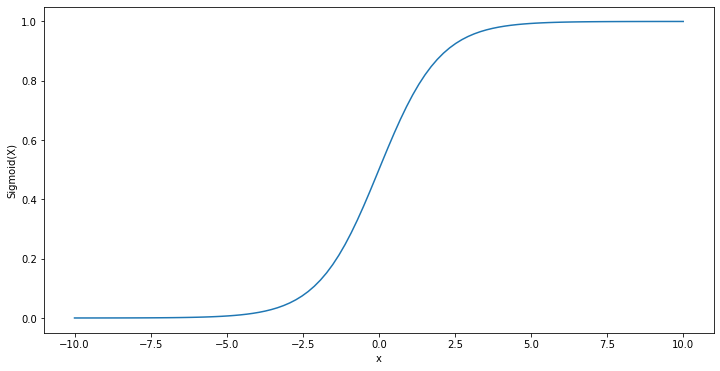
\includegraphics[scale=.5]{Imagens/sigmoid.png}
  	\caption{Logistic Regression curve}
  	\label{fig:sig}
\end{figure}

In Logistic Regression the best fitting line is estimated using the maximum likelihood method, which finds the coefficients for which the likelihood of observing the data is maximized. This method works by differentiating a likelihood function for each parameter to find the coefficients that maximize the probability of the observed data. There are no closed-form solutions for these differentiations, so iterative methods must be used. Iterative weighted least squares (see \cite{nelder1972generalized}) is an example of such a method.

The Logistic Regression method offers some interpretations that are easy to understand. The $y$ axis can be interpreted as the probability $\pi(x)$ that some instance $x$ belongs to the default class. For example, if the problem is to classify if a picture has a cat, $y=1$, the default class, could represent that the picture has a cat, while $y=0$ that the picture has no cat. The probability that an input $x$ belongs to a default class ($y=1$) could be stated as:

\begin{equation} \pi(x) =\pi(y=1|x). \end{equation}

The logistic regression model, where $\beta_0$ and $\beta_1$ are the coefficients, is defined by the following equation:

\begin{equation} \label{eqn} \pi(x) = \frac{e^{\beta_0+\beta_1x}}{1+e^{\beta_0+\beta_1x}}, \end{equation}

Equation \eqref{eqn} works in the case where the input has only one attribute. In the multi-attribute case, to each attribute, a coefficient is generated. Besides that, another important equation is the \emph{logit} transformation:

\begin{equation} g(x) = ln\frac{\pi(x)}{1-\pi(x)} = \beta_0+\beta_1x, \end{equation}

This ratio in the middle is called the \emph{odds} of the default class. Odds are an important concept that can be defined as the probability that an event occurs divided by the probability that the event does not occur. When odds > 1 the event is more likely to occur, and when odds < 1 the event is more likely to not occur.

The logit $g(x)$ has several attractive properties of the linear regression model, such as linearity, continuity, and range from negative to positive infinity. The coefficient $\beta_0$ (intercept) can be interpreted as assuming a value of 0 for all the predictors in the model. Further, the coefficient $\beta_1$ (slope) can be interpreted as the change in the response variable for every unit increase in the predictor. In short:

\begin{equation} \beta_1 = g(x+1) - g(x) \end{equation}

In summary, the algorithm for the Logistic Regression classifier is:

\begin{algorithm}[H]
Step 1 - Use a maximum likelihood method to find the logistic regression function's coefficients. \\
Step 2 - Plug in the values of the new instances' attributes. \\
Step 3 - The result class will be the default class (Y=1) if the probability is closer to 1. Otherwise, it will be the other class (Y=0). 
\caption{Logistic Regression}
\end{algorithm}

\section{Clustering}

Clustering is a technique that groups similar objects. It is useful to extract information from unlabeled data. One of the common methods of clustering is the $k$-means \cite{bramer2007principles}.

\subsection{$k$-Means}

The first step in the $k$-means method is to decide how many clusters will be created from the data. This is the $k$ value. To build the $k$ clusters an objective function is chosen to measure the quality of the set of clusters. This function can be the sum of the squares of the distances of each point from the centroid, i.e center, of the cluster to which it belongs. The value of this function should be minimal.

Next, $k$ points are selected as the centroids of $k$ potential clusters. These points can be selected in any desired way, but it is usually better to choose $k$ initial points that are far apart. Then, each point is added to the nearest centroid one by one. After all objects have been assigned, the centroids are recalculated and the previous steps are repeated until the centroids remain unchanged.

\section{Model training and performance evaluation}
\label{sc:training}

In the process of creating models, there are two distinct phases: building and evaluating the models. The data set for each of these phases is a partition of the original data set. This way, there are at least two sets: the training set, for building the model; and the testing set, for the evaluation. In the building phase, the classifiers' algorithms aim to create a function that best maps the data attributes to data classes, while the testing phase looks to evaluate the predictive aspect of the model to new data not previously seen \cite{cechinel2020mineraccao}.

The following section \ref{sc:dp} shows the common ways of partitioning the data set, section \ref{sc:ht} presents a method used to improve the classifiers' performance, and, finally, section \ref{sc:pm} shows ways to evaluate the performance of the DM algorithms.

\subsection{Data partitioning}
\label{sc:dp}

There are different ways that the data set can be partitioned into training and testing sets. In some cases, it already exists some natural way of dividing the data set. For example, if we wish to build a model to classify students by either pass or fail in a class, given that this class was offered in distinct semesters, we could test the data with some semester $A$ and train the data with the remaining semesters. When there is not an obvious way to divide the data, the alternative is to use some data partitioning technique. Holdout and k-fold cross-validation are the two main methods to partition the data.

\subsubsection{Holdout}

The holdout method randomly divides the data into two sets that do not overlap. It is common to use 75\% of data for training and 25\% for testing, but this is not a universal rule. This method is usually used when the data set has a large number of samples.

\subsubsection{K-fold cross-validation}

The k-fold cross-validation method is a type of validation that splits the data set into k folds and uses k-1 folds for training and the remaining fold for testing. This procedure is repeated k times so that each fold has been used for testing exactly once. Finally, the performance metrics are calculated based on the average performance of those repetitions. A common number of folds used in real applications is 10, a so-called 10-fold. It is usually used when the data set has a limited amount of samples.

\subsection{Hyperparameter tuning}
\label{sc:ht}

The DM algorithms often have parameters that can be adjusted to develop the most optimal model. These are called hyperparameters. A popular technique used in hyperparameter selection is grid search. In this approach, the parameters of the classifiers are exhaustively searched through a manually specified subset of the possible values to those parameters.

\subsection{Performance metrics}
\label{sc:pm}

Considering the characteristics of each data set and which model was used, different metrics can be used for model evaluation. This section presents the most common metrics for the evaluation of classifiers.

\subsubsection{Confusion matrix}
When working on a classification problem it is common to divide the data set into two classes. In this situation, the predictive performance of the model can be described in a 2x2 matrix that is called a binary confusion matrix. This matrix has labels for the real and observed classes of the data. Hence, there are four possible combinations: true-positive (TP) and true negative (TN), relating to the correct answers; false-positive (FP) and false negative (FN), relating to the incorrect answers, as can be seen in table \ref{tab:cm}.

\begin{table}[htb]
\centering
\begin{tabular}{cccc}
\hline
\multirow{2}{*}{} & \multirow{2}{*}{} & \multicolumn{2}{c}{Actual value} \\ \cline{3-4} 
 &  & True & False \\ \hline
\multirow{2}{*}{Model prediction} & True & True Positive (TP) & False Positive (FP) \\ \cline{2-4} 
 & False & False Negative (FN) & True Negative (TN) \\ \hline
\end{tabular}
\caption{Binary confusion matrix}
\label{tab:cm}
\end{table}

\subsubsection{Accuracy}

Accuracy is often used as a performance metric of classifiers. It measures the rate of correctly classified instances. Formally:

\begin{equation} Accuracy = \frac{number\ of\ correct\ predictions}{total\ number\ of\ predictions} \end{equation}

When dealing with a binary classification problem, it can also be defined as:

\begin{equation} Accuracy = \frac{TP+TN}{TP+TN+FP+FN} \end{equation}

\subsubsection{Precision}

Precision is the ratio between the correctly classified as true instances and all instances classified as true. This metric is also called Positive Predictive Value. Formally:

\begin{equation} Precision = \frac{TP}{TP+FP} \end{equation}

\subsubsection{Recall}

Recall is the ratio between the correctly classified as true instances and all true instances. This metric can also be called as True Positive Rate or Sensitivity. Formally:

\begin{equation} Recall = \frac{TP}{TP+FN} \end{equation}

%\subsubsection{True Negative Rate (TNR)}

%The\abrv{True Negative Rate}{TNR}TNR is the ratio between the correctly classified as false instances and all false instances. This metric is also called Specificity. Formally:

%\begin{equation} TNR = \frac{TN}{TN+FP} \end{equation}

\subsubsection{F-Measure}

The F-Measure combines Precision and Recall by calculating the harmonic average of them, which is the multiplicative inverse of the arithmetic mean of the multiplicative inverses of a set of values. This is done to avoid biased comments in the evaluation of models by using Precision or Recall separately. Formally defined as: 

\begin{equation} F\mbox{-}Measure = 2*\frac{Precision*Recall}{Precision+Recall} = \frac{2TP}{2TP+FP+FN} \end{equation}

